
\ifdefined\included
\else
\setcounter{chapter}{0} %% Numéro du chapitre précédent ;)
\dominitoc
\faketableofcontents
\fi

\chapter{Introduction}
\minitoc

To introduce this thesis and provide a global picture of its content, we first narrate a short story about a robot in a store. This story will then be used to identify some of the mains abilities a robot need to interact with humans with a focus on the knowledge it needs. While this thesis is from a roboticist point of view, working on interaction naturally leads to the study of cognitive psychology. From this field, we want to present an overview of the knowledge organisation models that have had an impact on the field, at the point to be now used for robotic researches.

\section{A prototypical scenario}

A company selling cameras have recently invested in a robot to support its employees in its stores. Their goal with these robots is to helps the employees during their daily tasks in the stores. The robots can prepare commands, put items on the shelves, cash customers, or advise them.

Max is one of these robots. It is a Pr2 design equipped with a head, two arms, and a mobile base with wheels. It is 9 a.m. and the robotic company having produce Max, power it on for the first time in the store. The robot starts navigating in the store, looking at all the products on the shelves. Liam, the human employee is counting the cash register when a customer enters the store. This customer is Tony. He looks to some cameras exposed on the shelves, going from one shelf to another.

Max, seeing Tony looking at all the cameras and Liam occupied to count the cash register, decides to go to see if the customer needs help.

\begin{quote} 
\centering 
\textit{
- "Hi, I am Max. Have you found a camera interesting you or do you need some advice?" \\
- "Hi, I don't really know anything about cameras. I go on a trip in a month and I would like a camera to take animal pictures during the trip." }
\end{quote}

For an amateur, Max chooses to present to Tony some automatic models. Moreover, since it is for a trip, he advises Tony to prefer a small camera. Looking at the prices, the customer explains that he did not want to spend more the 500 euros. Max thus select three options for him:

\begin{quote} 
\centering 
\textit{
- "You have this one at 350, the small black one here in front of you at 475, and on the other shelf there the small brown one near to the screen at 230." }
\end{quote}

\begin{figure}[h!]
\centering
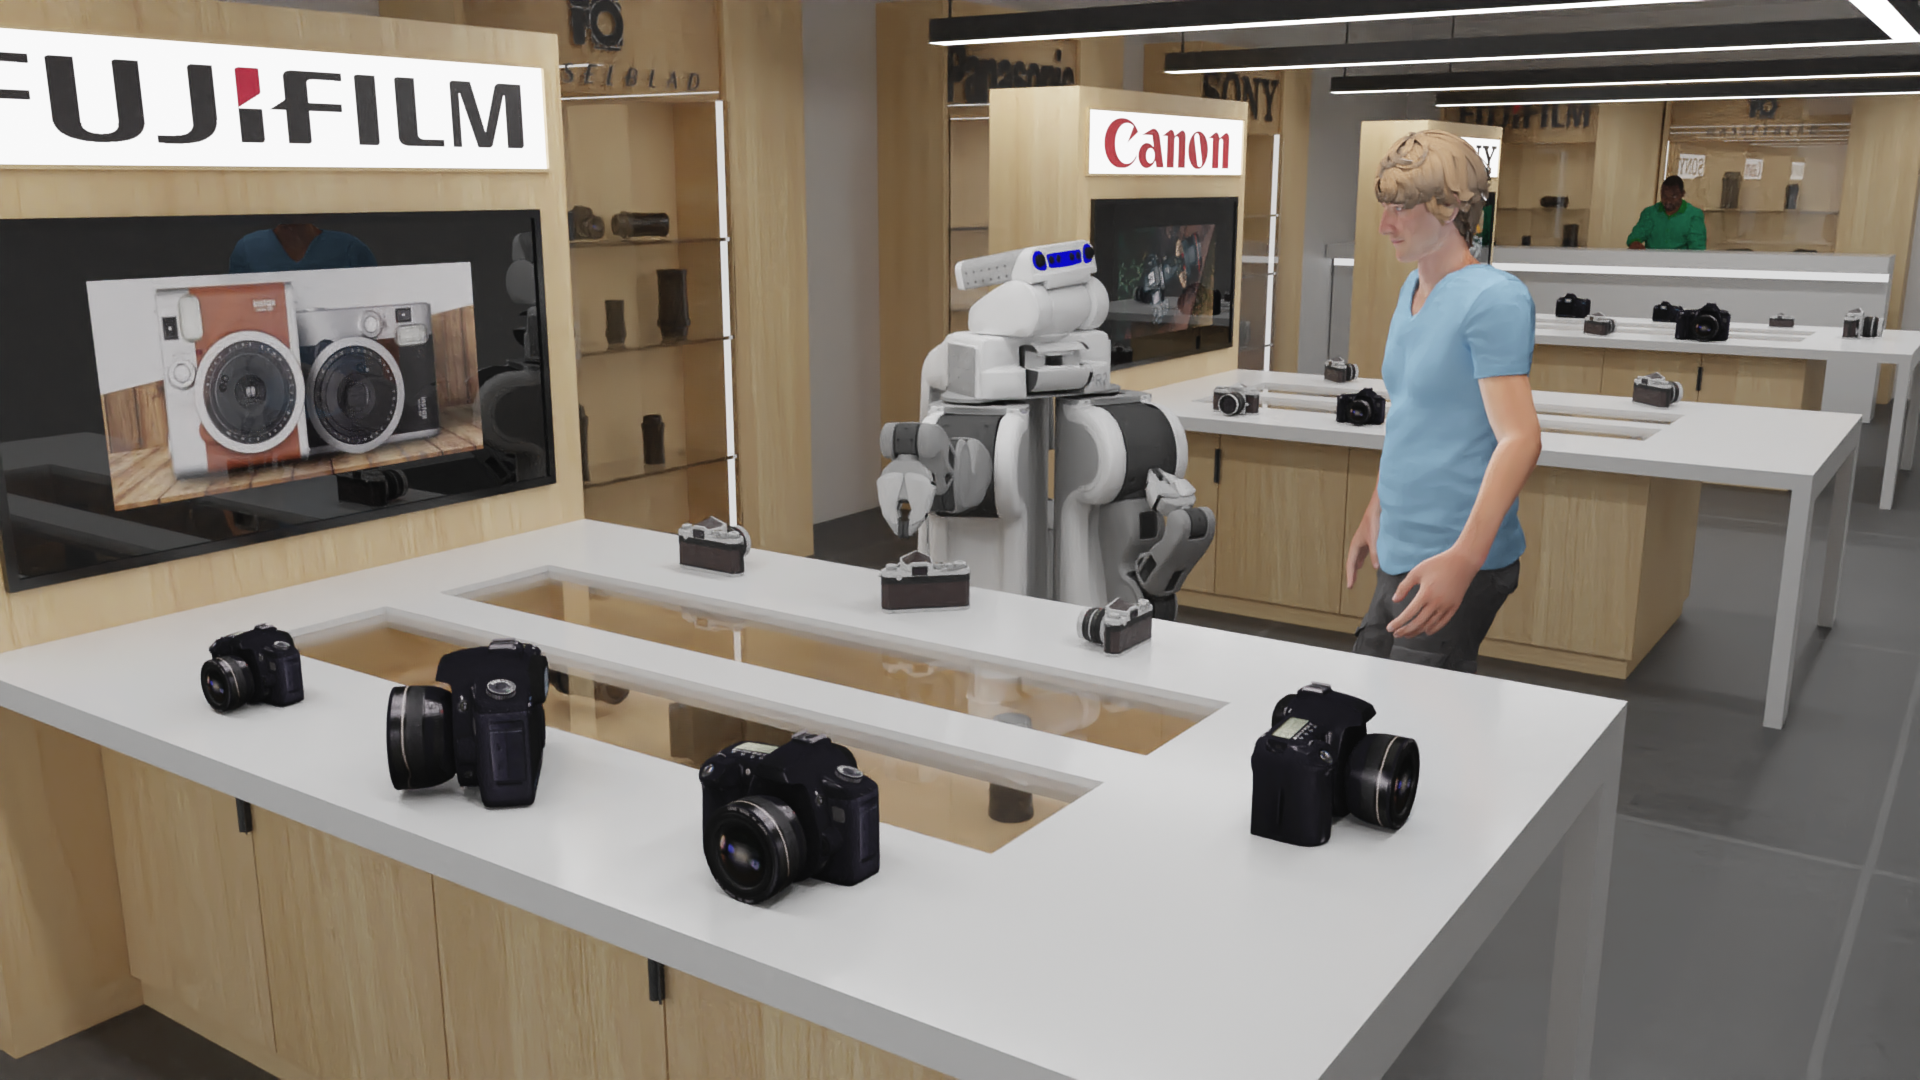
\includegraphics[width=\textwidth]{figures/introduction/camera_store_2.png}
\caption{\label{fig:cam_store} A Pr2 robot, as an employee of a camera store, advises a customer. }
\end{figure}

Explaining that, Max point to the cameras. They continue to discuss when Tony's phone rings. He has to go to join his wife. In another store in the mall. Not knowing where the other store is he said:

\begin{quote} 
\centering 
\textit{
- "I am sorry I have to go. I will come back in the week. I have to go to a store selling video game but I do not remember the name." \\
- "There is only one store selling video games in this mall, it is Game-ania." \\
- "Do you know how to reach it from there ?" \\
- "For sure"}
\end{quote}

Max slowly moves next to the entrance, followed by Tony. It raises one arm pointing to the aisle and said:

\begin{quote} 
\centering 
\textit{
- "Go down this aisle then turn left straight after the salad bar. After that Game-ania will be on your right when we walk."}
\end{quote}

Tony goes and come back the next morning. Max recognizing him, goes towards him. It asks Tony if he easily found the video game shop and recall the camera identified the day before.

\begin{quote} 
\centering 
\textit{
- "Yesterday we stop on two Fujifilm cameras and a Canon for your trip."}
\end{quote}

They continue to discuss and finally Tony selects the camera at 350 euros. Following Max's advice, takes a memory card and a second battery to have enough storage and power during his trip. In addition, he takes a lens to take pictures of animals from far. Unfortunately, the wanted camera is not available at the moment. The last in the store is the demonstration one. Max purpose to Tony to command it. The client agrees and goes.

A few days later, before opening, several boxes arrive at the store. Liam, the human employee, and Max have to open them, fill the stocks and prepare Tony's command. This is the first time since Max arrival they have to do it. They both go to the backroom to do this task together. There are two boxes. Liam starts opening one so Max starts opening the other. Max informs Liam about the camera which should arrive.

\begin{quote} 
\centering 
\textit{
- "Tell me if their is a X-T100, a customer commands one."}
\end{quote}

\begin{figure}[h!]
\centering
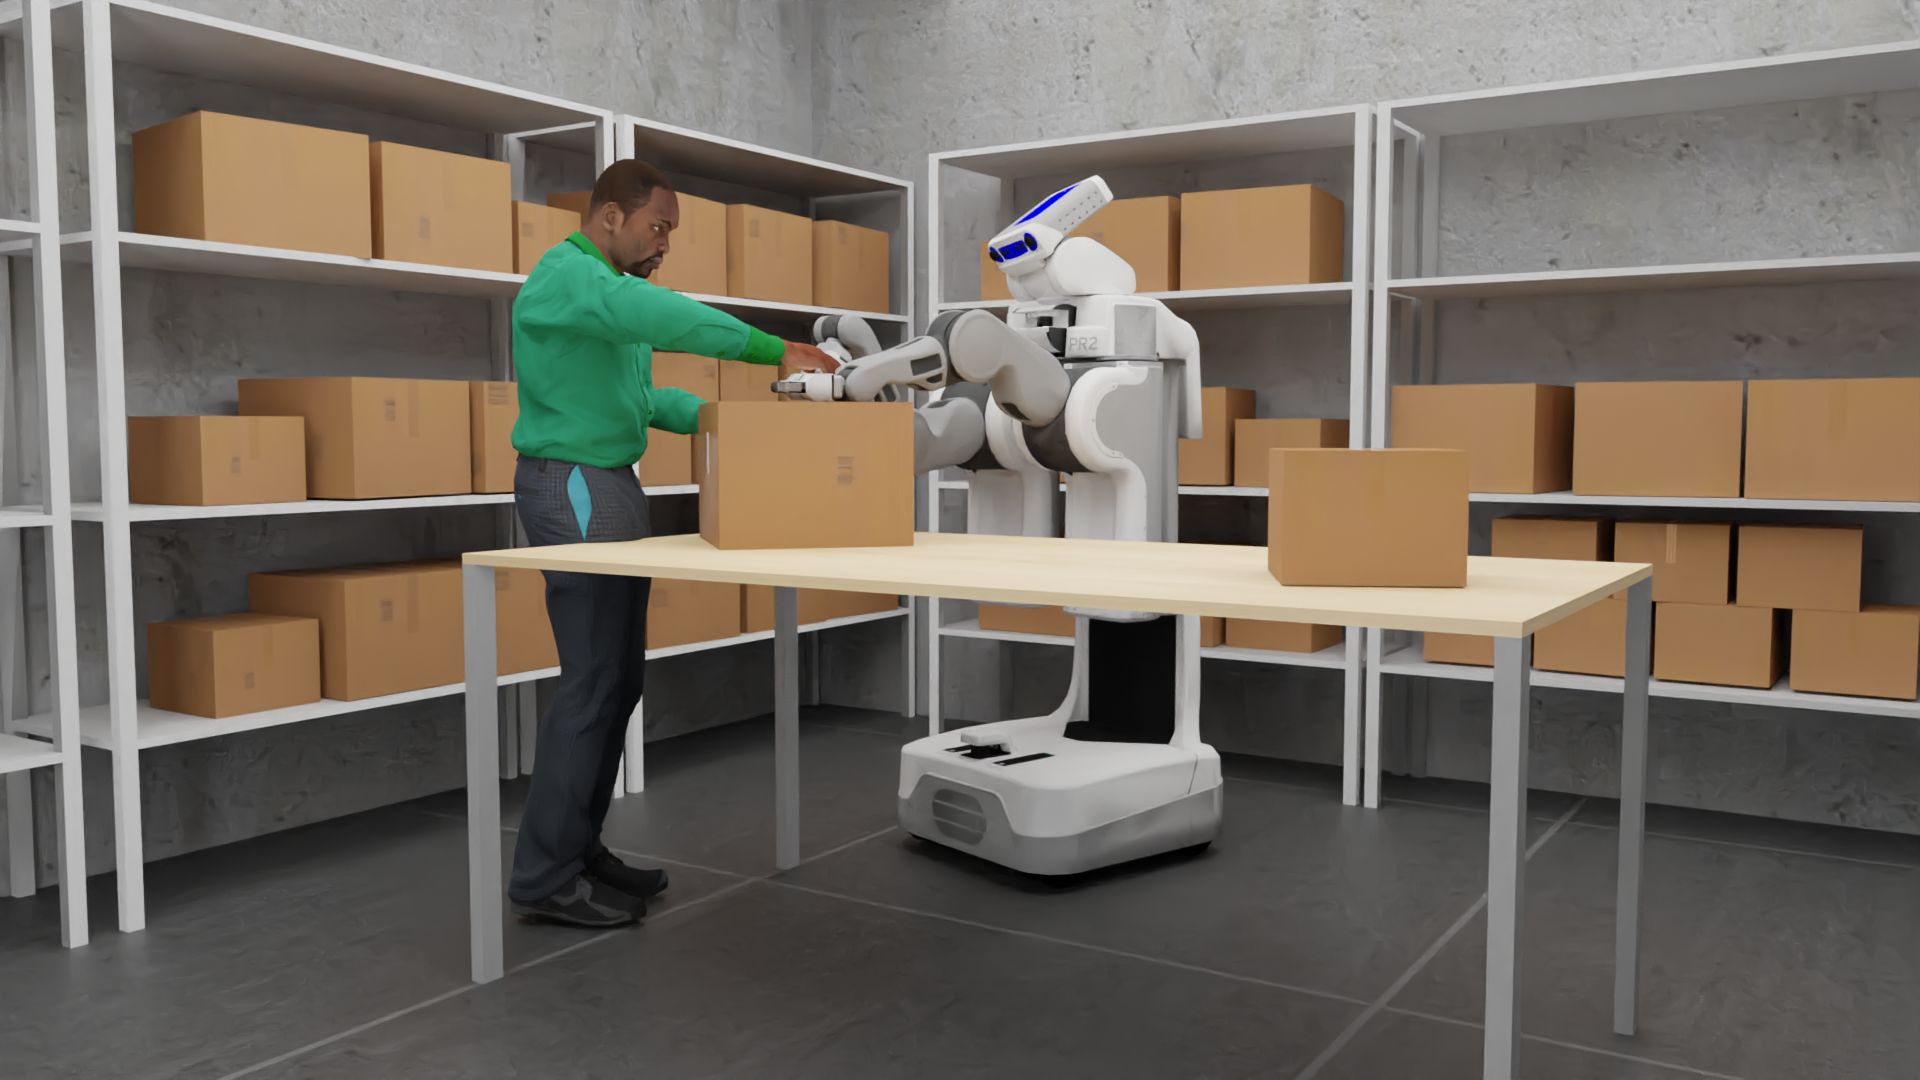
\includegraphics[width=\textwidth]{figures/introduction/camera_store_3.png}
\caption{\label{fig:cam_store} A Pr2 robot and a human employee collaborating to close a box. }
\end{figure}

Liam finds the camera. The robot explains to him that it also need an SD card of 32Go and a lens XC 15-45mm. It informs the human that the SD cards are too small for it to grasp them. It thus purposes to Liam to take some of the cameras to put on the shelves and to bring back the card and the lens at the same time. During this time, Max takes a box, put the camera in and the battery. When Liam comes back, he put the two other items in the same box. Then, Max maintains the box close while Liam scotch it. When finished, they both take the last items to put on the shelves and go to the main room.

The afternoon of the same day, Max is cashing in a customer. Tony enter is the store. Seeing him, it request Liam:

\begin{quote} 
\centering 
\textit{
- "Can you bring the command we prepared this morning? The client it is for is the one just entering, with the blue T-shirt."}
\end{quote}

Liam goes into the back room and brings back the correct box. Max cash the customer how finally get his camera in the time.

\section{Interacting with a robot: What can we expect ?}

\section[Knowledge organization]{Knowledge organization: Drawing inspiration from cognitive psychology }

Even if our goal in robotics is not to create a copy of the human, either in terms of body shape or cognition, drawing inspiration from it is nevertheless important. In the same way that roboticists take inspiration from the human body to create robots able to evolve in a world created by and for the human, the field of cognitive robotics takes inspiration of the human cognition to create robots able to interact with humans. While we do not aim to make a copy of human cognition, we think that a robot must endow similar capabilities if we want them to interact with us efficiently and in an acceptable way.

Regarding the knowledge representation, the first experimental study has been realized in 1885 by Ebbinghaus~\cite{ebbinghaus_1885_gedachtnis}. Since then, the definition of memory as the capacity to encode, store, and retrieve knowledge \cite{roediger_1996_retrieval} has been widely accepted. At the same time, the word "memory" has become a generic term suggesting a unique system. However, the human memory can rather be seen as several sub-systems that differ from their storage duration, storage capacity, and the level of consciousness necessary for information retrieval. In the rest of the section, we present some memory models, presented in a non-chronological way, and focussing on what is called long-term memory. During all this section, it is important to keep in mind that we only present models aiming to understand human cognition with a focus on knowledge management. No formal truth is stated here given that there is no consensus in the field. The presented models and terms will allow us to better understand the existing robotic cognitive architectures and give inspiration for the design and structuration of the components developed during this thesis.

\improvement{schema pour chaque model ?}
The primary division of the memory is done concerning the storage duration and capacity. From there has been defined the \textbf{short-term memory} (STM) and the \textbf{long-term memory} (LTM) \cite{atkinson_1966_some}. Short-term memory is characterized by its small capacity and its capability to retrieve information that has just been seen. We often hear about twenty seconds and seven items (or chunks)\improvement{ref}. Long-term memory, on the opposite, refers to any situation where we use information that has not just been seen. We often hear about infinite capacity and duration. It is this latter that allows the acquisition of new knowledge and the retrieval of information acquired a long time ago.

Over the years, what was called short-term memory has become the \textbf{working memory} (WM) \cite{baddeley_1986_dementia}. This change has been made to add a notion of knowledge manipulation. Instead of focusing on the only temporal aspect, it reflects its functional aspect. It is thus a system that retains information for the time necessary for its use by other cognitive functions. The working memory and the long-term memories are two independent but related systems. For information to be stored in long-term memory, we think that it has to pass by the working memory.

For the structure of the long-term memory, a first dichotomy is proposed by Graf and Schacter \cite{graf_1985_implicit} with the \textbf{implicit} and \textbf{explicit} memory. It reflects the way knowledge can be retrieved. Knowledge from explicit memory can be retrieved consciously and voluntarily. On the opposite, knowledge from the implicit memory is retrieved in situations in which our comportments are influenced by an experience. This is the case when you pour water into a glass. We do not need to retrieve explicitly how to perform this task. It is our experience that influences how we do it.

Another dichotomy has been proposed by Squire and Cohen \cite{squire_1982_remote} with the \textbf{procedural} and \textbf{declarative} memory. Procedural memory is the system allowing us to retain knowledge about our cognitive, motor, or perceptual skills. It is the memory of the know-how. A particularity of this memory is that it is difficult to speak about the knowledge it stores and we use them unconsciously. The declarative memory stores representations of facts, events, general knowledge, and memories of past events. This knowledge can be retrieved consciously and we can speak about them. Taking the example of the code of your credit card. Initially, this knowledge is store in the declarative memory. When you need it you can easily remember it at say it. The more you use it and it slowly becomes an automatism. It became hard to remember it consciously while you use it every day and if you need to say it you can type it on a virtual keyboard to remember it. It has slowly moved into your procedural memory. We see that both dichotomies are almost equivalent. The declarative memory of Squire is related to the implicit memory of Graf, and the procedural one is related to the implicit memory.

Going deeper into the declarative memory, Tulving has proposed a dichotomy between \textbf{episodic} and \textbf{semantic} memory \cite{tulving_1995_organization}. The episodic memory retains knowledge related to past experienced events, which are specific to our individual experience, and localized both in space and time. The semantic memory is more general and retains knowledge that we accumulate all along with our life concerning our environment. It can be seen as an encyclopedic memory independent of the acquisition context. While the episodic memory is related to "remembering", the sematic one is related to "knowing". Taking as an example your visit to Toulouse \footnote{If you never visit it, you can take another city you have visited but you should plan to visit it anyway.}, this visit is encoded in the episodic memory while the knowledge that Toulouse is a city in France is encoded in the semantic one.

\begin{figure}[h!]
\centering
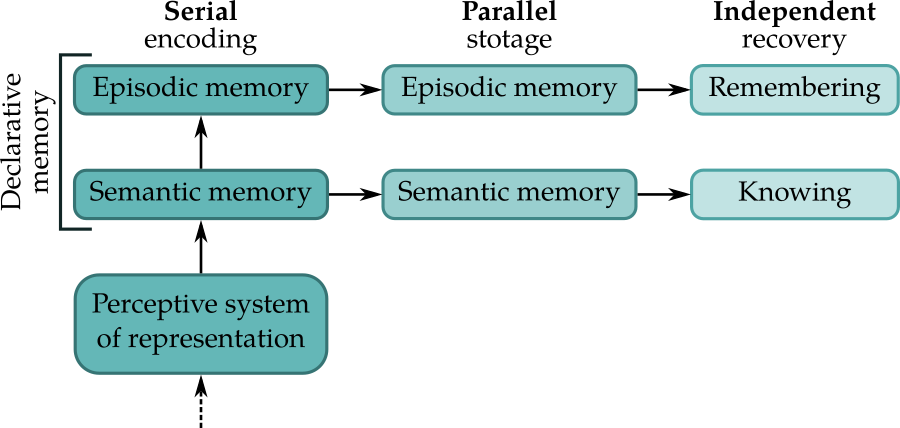
\includegraphics[scale=0.45]{figures/introduction/SPI.png}
\caption{\label{fig:SPI} Relations between episodic memory and semantic memory according to the SPI (Serial, Parallel, and Independent) model of Tulving (1995).}
\end{figure}

With the previous example, we saw that even if these two sub-systems of the declarative memory are independent, they are therefore in interaction with eachother as we can apply a semantic treatment on the episodic memory. To better undertand their relation, Tulving has proposed Serial, Parallel, and Independent model (SPI). As illustrated in Figure~\ref{fig:SPI}, the encoding of an information is serial (S) passing first by the semantic memory then in the episodic one. The storage in both memories is performed in parallel (P). Finally, the information recovery is independy between the two memories.
As we explain in the begin of this section, the presented theory can not be proven and must therefore be taken as~\cite{tulving_1995_organization} "an explicit starting point for a more systematic pursuit of what is clearly the next problem that needs to be tackled".

\section{Contributions}

\subsection{Knowledge representation}

\subsection{Knowledge exploitation}

\section{A reader's guide}


